\documentclass[11pt]{beamer}
\usetheme{Warsaw}
\usepackage[utf8]{inputenc}
\usepackage[portuguese]{babel}
\usepackage[T1]{fontenc}
\usepackage{amsmath}
\usepackage{amsfonts}
\usepackage{amssymb}
\usepackage{graphicx}
\author{Leandro, Diego e Alexandre}
\title{k-Nearest Neighbors algorithm (KNN)}
%\setbeamercovered{transparent} 
%\setbeamertemplate{navigation symbols}{} 
%\logo{} 
%\institute{} 
%\date{} 
%\subject{} 
\begin{document}

\begin{frame}
\titlepage
\end{frame}

\begin{frame}
\tableofcontents
\end{frame}

\section{Introdução}

\begin{frame}{Objetivo}
	\begin{itemize}
	\item Realizar um estudo sobre a aplicação do algoritmo KNN em FPGAs;
	\item Reconhecimento de indivíduos a partir dos movimentos e dados
	antropométricos \cite{granaidentificaccao};
	\item Foi realizado uma conexão entre o Kinect, a placa Altera Cyclone
	(2C35) e o computador para coleta em tempo real dos dados;
	\item Construido um ambiente experimental simulado. 
	\end{itemize}
\end{frame}

\section{Processo de implementação do algoritmo KNN em VHDL}

\begin{frame}{Descrição do bloco operativo}
	\begin{itemize}
	\item O bloco operativo é dividido basicamente em 3 loops;
	\item Os pontos recebidos pela parte de aquisição de dados vem no padrão
	IEEE 754;
	\item Megafunctions:
		\begin{itemize}
		\item Memória
		\item Subtrator
		\item Somador
		\item Multiplicador
		\item SQRT
		\item Comparador de ponto flutuante
		\end{itemize}
	\end{itemize}
\end{frame}

\begin{frame}{Descrição do bloco operativo}
	\begin{itemize}
	\item Memória
	\begin{figure}[ht]
	\centering
	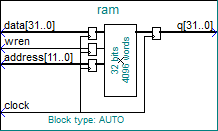
\includegraphics[width=.5\textwidth]{ram}
	\label{fig:ram}
	\end{figure}
	\end{itemize}
\end{frame}

\begin{frame}{Descrição do bloco operativo}
	\begin{itemize}
	\item Somador - Subtrator
	\begin{figure}[ht]
	\centering
	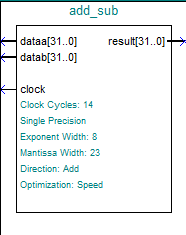
\includegraphics[width=.5\textwidth]{add_sub}
	\label{fig:add_sub}
	\end{figure}
	\end{itemize}
\end{frame}

\begin{frame}{Descrição do bloco operativo}
	\begin{itemize}
	\item Multiplicador
	\begin{figure}[ht]
	\centering
	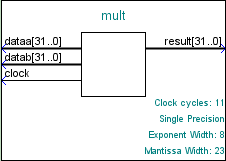
\includegraphics[width=.5\textwidth]{mult}
	\label{fig:mult}
	\end{figure}
	\end{itemize}
\end{frame}

\begin{frame}{Descrição do bloco operativo}
	\begin{itemize}
	\item Raiz quadrada
	\begin{figure}[ht]
	\centering
	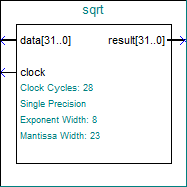
\includegraphics[width=.5\textwidth]{sqrt}
	\label{fig:sqrt}
	\end{figure}
	\end{itemize}
\end{frame}

\begin{frame}{Descrição do bloco operativo}
	\begin{itemize}
	\item Compara se dataa é menor que datab
	\begin{figure}[ht]
	\centering
	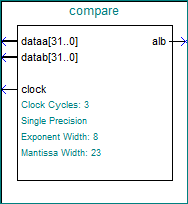
\includegraphics[width=.5\textwidth]{compare}
	\label{fig:compare}
	\end{figure}
	\end{itemize}
\end{frame}

\begin{frame}{Descrição do bloco operativo}
	\begin{figure}[ht]
	\centering
	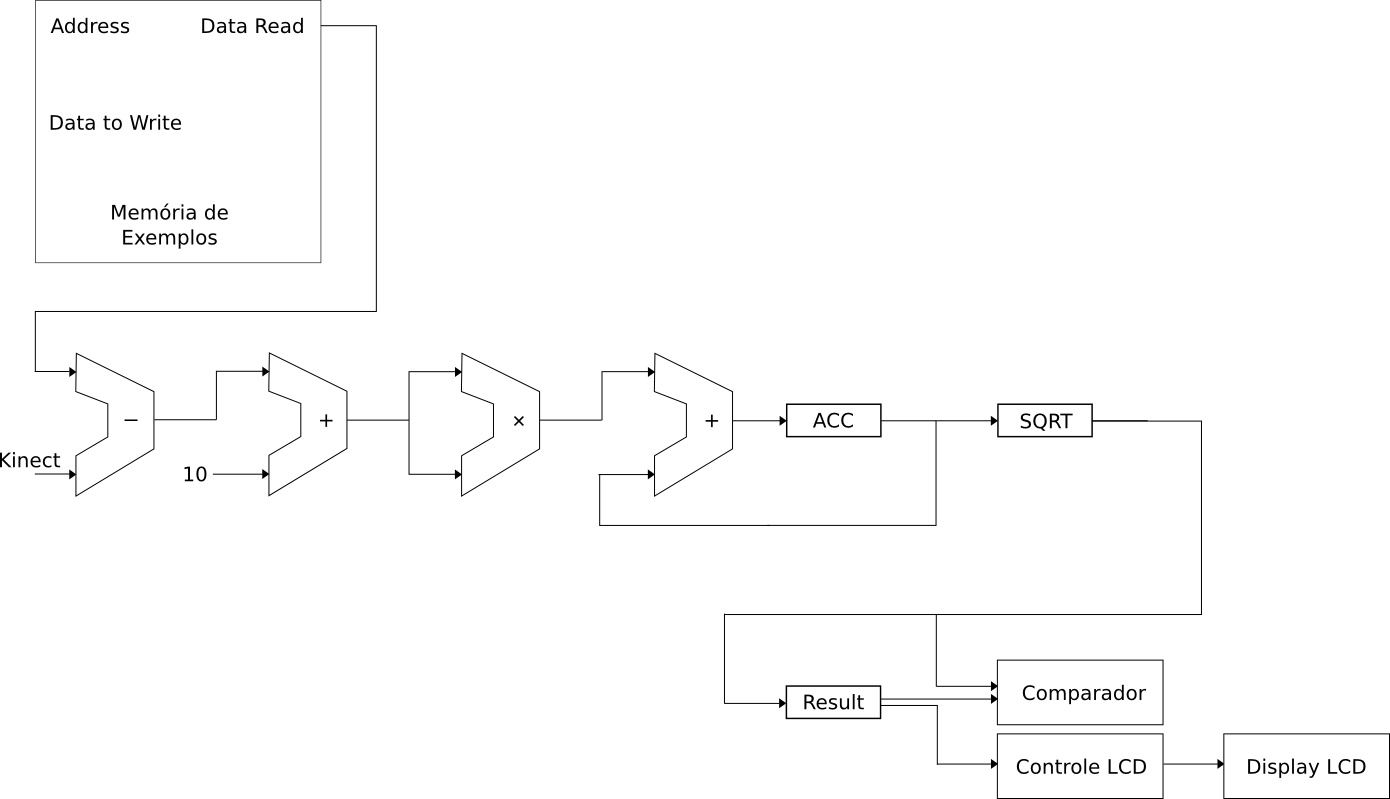
\includegraphics[width=1.0\textwidth]{knn_sem_controle}
	\label{fig:knn_sem_controle}
	\end{figure}
\end{frame}

% LEANDRO SÓ COPIA O TRECHO DE CÓDIGO ABAIXO PARA CIRAR UM NOVO SLIDE
\begin{frame}{Descrição do bloco de controle}
	\begin{itemize}
	\item Bloco de controle
	\end{itemize}
\end{frame}
% FIM DA IMPLEMENTAÇÃO DO CALCULO DO KNN

\section{Resultados}
\begin{frame}{Resultados}

\begin{itemize}
	\item Resultados
\end{itemize}

\end{frame}

\section{Referências}
\begin{frame}{Referências}
  
	\bibliography{ref}{}
	\bibliographystyle{plain}

\end{frame}

\end{document}